\subsection{Ender-3 V2}

The Creality Ender-3 V2 is a widely used consumer-grade 3D printer that has become a standard platform in education, prototyping, and hobbyist communities. This device is designed to provide an accessible entry point into 3D printing with its

\begin{itemize}
    \item Affordable price point,
    \item User-friendly design
    \item Straightforward assembly process, and
    \item Strong community support,
\end{itemize}

while still offering sufficient flexibility and performance for more advanced users.

\begin{figure}[H]
    \centering
    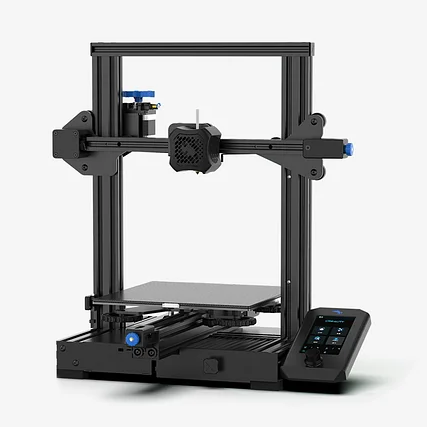
\includegraphics[width=0.5\textwidth]{components/image/ender3v2_product.png}
    \caption{Creality Ender-3 V2 3D printer \cite{ender3v2_creality}.}
    \label{fig:ender3v2_product}
\end{figure}

The Ender-3 V2 operates using Fused Deposition Modeling (FDM) technology, a process in which thermoplastic filament is melted and deposited layer by layer to create three-dimensional objects \cite{fdm_3dsourced}. It supports common materials such as PLA, ABS, and PETG, making it suitable for both simple prototypes and functional mechanical parts. 

The printer features a build volume of approximately 220 × 220 × 250 mm and features a partially modular design and is typically shipped as a semi-assembled kit, requiring users to complete the assembly process themselves. This aspect is particularly valuable in educational contexts, as it helps users understand the mechanical and electronic components of the system.

An important characteristic of the Ender-3 V2 is its strong community support and upgrade ecosystem. Users can modify and enhance the printer with various upgrades, such as automatic bed leveling sensors, improved extruders, or custom firmware. This extensibility makes it an excellent platform for experimentation and learning, particularly for students interested in mechanical design, electronics, and embedded systems.